% RDM truncation, told as a row of equalities. Companion to imgs/rtm_trunc_row.tex, and the
% defence-local expansion of thesis Figure 13 (imgs/truncation.pdf): the thesis draws only the
% first and last member of the chain, this one draws the collapse in between.
%
% (a) the canonical condition: a tensor contracted with its conjugate over the physical index and
%     the left virtual index is the identity on the remaining index.
% (b) the derivation: the traced block right of the cut collapses column by column through (a);
%     the open block left of the cut groups into one isometry U and its conjugate U^dagger; the
%     spectrum that survives is carried by the centre tensor M alone.
% In every sub-diagram the bonds are drawn first and the tensors on top, so no leg crosses a shape.
%
% Standalone: compiles to imgs/rdm_trunc_row.pdf.
\documentclass[tikz,border=3pt]{standalone}
\usepackage{amsmath,amssymb,braket,graphicx}
\usetikzlibrary{arrows.meta,shapes.geometric}

\definecolor{tnL}{RGB}{243,116,63}      % the centre tensor, conjugate row
\definecolor{tnLl}{RGB}{250,190,150}    % the centre tensor, ket row
\definecolor{tnR}{RGB}{60,110,150}      % chain tensors, conjugate row
\definecolor{tnRl}{RGB}{160,195,220}    % chain tensors, ket row

\newcommand{\DX}{0.56}
\newcommand{\ST}{0.34}
\newcommand{\HA}{0.36}   % half separation between the ket row and its conjugate

\newcommand{\Dhh}{0.19}   % half-height of a tensor
\newcommand{\Dbb}{0.19}   % straight body, so the D comes out as wide as it is tall

% a D-shaped tensor centred at (#1,#2), flat edge on the left, filled #3
\newcommand{\dR}[3]{%
  \filldraw[fill=#3, draw=black, line width=0.95pt]
    ({#1-(\Dbb+\Dhh)/2},{#2-\Dhh}) -- ({#1+(\Dbb-\Dhh)/2},{#2-\Dhh})
    arc[start angle=-90, end angle=90, radius=\Dhh]
    -- ({#1-(\Dbb+\Dhh)/2},{#2+\Dhh}) -- cycle;}

% the orthogonality centre, drawn as a square as in the thesis figure
\newcommand{\sq}[3]{%
  \filldraw[fill=#3, draw=black, line width=0.95pt]
    ({#1-\Dhh},{#2-\Dhh}) rectangle ({#1+\Dhh},{#2+\Dhh});}

% grouped isometry: one wide tensor carrying the comb of physical legs it absorbed
% #1 x, #2 y, #3 fill, #4 comb direction (+1 above, -1 below)
\newcommand{\wideD}[4]{%
  \filldraw[fill=#3, draw=black, line width=0.95pt]
    (#1,{#2-\Dhh}) -- ({#1+0.46},{#2-\Dhh})
    arc[start angle=-90, end angle=90, radius=\Dhh] -- (#1,{#2+\Dhh}) -- cycle;
  \foreach \c in {0.10,0.24,0.38} {
    \draw[bond] ({#1+\c},{#2+#4*\Dhh}) -- ({#1+\c},{#2+#4*(\Dhh+\ST)});
  }}

\newcommand{\bigpar}[1]{\scalebox{1.0}[3.4]{$#1$}}

\begin{document}
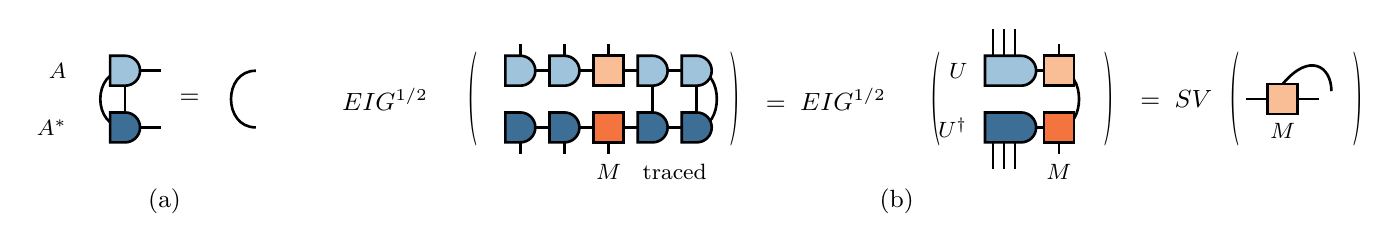
\begin{tikzpicture}[
    bond/.style={draw=black, line width=0.95pt},
    tag/.style={font=\small},
    idx/.style={font=\footnotesize},
  ]

  %% ================= (a) the canonical condition =================
  \begin{scope}[xshift=-3.30cm, yshift=0cm]
    \draw[bond] (0,\HA) .. controls (-0.42,\HA) and (-0.42,-\HA) .. (0,-\HA);
    \draw[bond] (0,\HA) -- (0,-\HA);
    \draw[bond] (0,\HA)  -- (0.46,\HA);
    \draw[bond] (0,-\HA) -- (0.46,-\HA);
    \dR{0}{\HA}{tnRl}
    \dR{0}{-\HA}{tnR}
    \node[idx, anchor=east] at (-0.62,\HA)  {$A$};
    \node[idx, anchor=east] at (-0.62,-\HA) {$A^{*}$};
    \node[tag] at (0.82,0) {$=$};
    \draw[bond] (1.66,\HA) .. controls (1.24,\HA) and (1.24,-\HA) .. (1.66,-\HA);
    \node[tag] at (0.5,-1.30) {(a)};
  \end{scope}

  %% ================= (b) the derivation, on one line =================

  %% ---- step 1: the reduced density matrix as it stands ----
  \node[tag] at (0,0) {$EIG^{1/2}$};
  \node at (1.12,0) {\bigpar{(}};
  \begin{scope}[xshift=1.72cm]
    \draw[bond] (0,\HA)  -- ({4*\DX},\HA);
    \draw[bond] (0,-\HA) -- ({4*\DX},-\HA);
    \draw[bond] ({4*\DX},\HA) .. controls ({4*\DX+0.34},\HA)
      and ({4*\DX+0.34},-\HA) .. ({4*\DX},-\HA);
    \foreach \i in {0,1,2} {                       % open: these legs are the matrix indices
      \draw[bond] ({\i*\DX},\HA)  -- ({\i*\DX},{\HA+\ST});
      \draw[bond] ({\i*\DX},-\HA) -- ({\i*\DX},{-\HA-\ST});
    }
    \foreach \i in {3,4} {                          % traced: ket leg tied to its conjugate
      \draw[bond] ({\i*\DX},\HA) -- ({\i*\DX},-\HA);
    }
    \foreach \i in {0,1} { \dR{\i*\DX}{\HA}{tnRl} \dR{\i*\DX}{-\HA}{tnR} }
    \sq{2*\DX}{\HA}{tnLl}  \sq{2*\DX}{-\HA}{tnL}
    \foreach \i in {3,4} { \dR{\i*\DX}{\HA}{tnRl} \dR{\i*\DX}{-\HA}{tnR} }
    \node[idx] at ({2*\DX},{-\HA-\ST-0.22}) {$M$};
    \node[idx] at ({3.5*\DX},{-\HA-\ST-0.22}) {traced};
  \end{scope}
  \node at (4.45,0) {\bigpar{)}};

  %% ---- step 2: (a) has eaten the traced block; the open block is one isometry ----
  \node[tag] at (5.60,0) {$=\;EIG^{1/2}$};
  \node at (7.00,0) {\bigpar{(}};
  \begin{scope}[xshift=7.62cm]
    \def\XC{0.94}
    \draw[bond] (0.46,\HA)  -- (\XC,\HA);
    \draw[bond] (0.46,-\HA) -- (\XC,-\HA);
    \draw[bond] (\XC,\HA) .. controls ({\XC+0.34},\HA)
      and ({\XC+0.34},-\HA) .. (\XC,-\HA);
    \draw[bond] (\XC,\HA)  -- (\XC,{\HA+\ST});
    \draw[bond] (\XC,-\HA) -- (\XC,{-\HA-\ST});
    \wideD{0}{\HA}{tnRl}{1}
    \wideD{0}{-\HA}{tnR}{-1}
    \sq{\XC}{\HA}{tnLl}  \sq{\XC}{-\HA}{tnL}
    \node[idx, anchor=east] at (-0.10,\HA)  {$U$};
    \node[idx, anchor=east] at (-0.10,-\HA) {$U^{\dagger}$};
    \node[idx] at (\XC,{-\HA-\ST-0.22}) {$M$};
  \end{scope}
  \node at (9.20,0) {\bigpar{)}};

  %% ---- step 3: U^dagger U = 1, so only the centre is left ----
  \node[tag] at (10.05,0) {$=\;SV$};
  \node at (10.80,0) {\bigpar{(}};
  \begin{scope}[xshift=11.40cm]
    \draw[bond] (-0.46,0) -- (0.46,0);
    \draw[bond] (0,0.19) .. controls (0.34,0.60) and (0.62,0.42) .. (0.62,0.10);
    \sq{0}{0}{tnLl}
    \node[idx] at (0,-0.40) {$M$};
  \end{scope}
  \node at (12.35,0) {\bigpar{)}};

  \node[tag] at (6.5,-1.30) {(b)};

\end{tikzpicture}
\end{document}
